\chapter{Makefiles}


\includegraphics[scale=0.20]{images/books-1163695_1920.jpg}

\justify{}
A Makefile\index{Makefile} is a handy way to put short sets of oft-repeated steps at the fingertips of the developer. Rather than
typing three complicated and possibly hard to recall strings to kick off your Docker container, you can simply type ``make docker'' and
have everything build as desired. We're going to be using GNU Make for our projects. 

\section{Parts of a Makefile}

A Makefile can be as simple as a few lines or grow to become and extremely intricate and vital piece of your build environment. 
You might like to have a look at \href{https://www.gnu.org/software/make/manual/make.html}{the GNU make manual} at least once
just to get a feel for all the things it can do for you.

\subsection{The PHONY Directive}

\justify{}
If a file or directory exists with the same name as a stanza in the Makefile, you will need to specify it under the \emph{PHONY} directive.
This will allow the Makefile to find and run the desired commands.

\justify{}
Consider this example, where we have three directories (docker, docs, and python) and we also have three Makefile directives of the same name:

\begin{mybox}{\thetcbcounter: The PHONY Directive}
	\lstinputlisting{code/06-makefiles/phony.txt}
\end{mybox}

\subsection{Targets}

\justify{}
Makefiles are comprised of various stanzas, know as targets. This is where the work gets done. Let's add a target for Docker and a target for
Python to make our lives easier in the future. Consider the two target stanzas below.

\justify{}
\begin{mybox}{\thetcbcounter: A Makefile Target}
	\lstinputlisting{code/06-makefiles/makefile-target}
\end{mybox}

\justify{}
When the user types make docker at the CLI to invoke the docker target in the Makefile, the fist thing that happens is the python target is
called. If the file python/requirements.txt exists, we attempt to install the modules listed within that requirements file using the
Python ``pip'' package manager. Once completed, the thread of execution returns to the docker target. A message is sent to the user via STDOUT
that we will be building with docker-compose. An empty file at the root of the containers filesystem named /.dockerenv is a convention that
indicates we are operating inside a containerized environment. After a quick check for existence of the file /.dockerenv, we use docker-compose
to build from our Dockerfile, and then start a BASH shell in our ``cloudlab'' container. The user now has the ability to run BASH commands
``inside'' the Docker container.

\justify{}
Be sure when you indent in a Makefile that you use tabs, not spaces. You can use the backslash character in a Makefile to combine two consecutive
lines into one logical line.

\section{A Simple Makefile Exmaple}

\justify{}
Let's look at a simple Makefile example. 

\section{Full Example Makefile}
\justify{}
Next, let's look at a full working example of a Makefile.

\section{Directory Structure with Makefile}
\justify{}
Relevant files and folders related to our Makefile are organized as seen
below.

\begin{figure}[!htb]
	
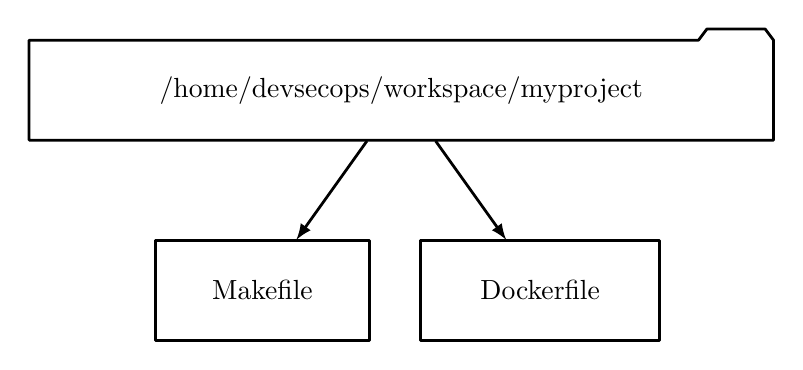
\begin{tikzpicture}[>=latex,line join=bevel,]
  \pgfsetlinewidth{1bp}
%%
\pgfsetcolor{black}
  % Edge: devsecops -> Makefile
  \draw [->] (121.64bp,71.697bp) .. controls (115.77bp,63.474bp) and (108.63bp,53.483bp)  .. (96.217bp,36.104bp);
  % Edge: devsecops -> Dockerfile
  \draw [->] (146.36bp,71.697bp) .. controls (152.23bp,63.474bp) and (159.37bp,53.483bp)  .. (171.78bp,36.104bp);
  % Node: devsecops
\begin{scope}
  \definecolor{strokecol}{rgb}{0.0,0.0,0.0};
  \pgfsetstrokecolor{strokecol}
  \draw (268.0bp,108.0bp) -- (265.0bp,112.0bp) -- (244.0bp,112.0bp) -- (241.0bp,108.0bp) -- (0.0bp,108.0bp) -- (0.0bp,72.0bp) -- (268.0bp,72.0bp) -- cycle;
  \draw (134.0bp,90.0bp) node {/home/devsecops/workspace/myproject};
\end{scope}
  % Node: Makefile
\begin{scope}
  \definecolor{strokecol}{rgb}{0.0,0.0,0.0};
  \pgfsetstrokecolor{strokecol}
  \draw (122.5bp,36.0bp) -- (45.5bp,36.0bp) -- (45.5bp,0.0bp) -- (122.5bp,0.0bp) -- cycle;
  \draw (84.0bp,18.0bp) node {Makefile};
\end{scope}
  % Node: Dockerfile
\begin{scope}
  \definecolor{strokecol}{rgb}{0.0,0.0,0.0};
  \pgfsetstrokecolor{strokecol}
  \draw (227.0bp,36.0bp) -- (141.0bp,36.0bp) -- (141.0bp,0.0bp) -- (227.0bp,0.0bp) -- cycle;
  \draw (184.0bp,18.0bp) node {Dockerfile};
\end{scope}
%
\end{tikzpicture}


	\caption{Makefile and related files.}
\label{makefile}
\end{figure}

